\section{Experiment 3: EVS resampling study}

In the third experiment, we performed a resampling study based on the EVS data to assess
how well the results obtained from Experiments 1 and 2 carried over to real data applications.
EVS is a large-scale, cross-national survey on human values administered in around 50 countries
across Europe.
It covers a wide range of human values regarding family, work, environment, perceptions of 
life, politics, society, religion, morality, and national identity.
EVS is a high-quality survey widely used for comparative studies between European countries.
Furthermore, it is accessible free of charge and it represents the type of data social scientist 
regularly analyze.
Variables in the EVS data are discrete numerical and categorical items following a 
variety of distributions.

In Experiment 3, we treated the original EVS data as the population from which we drew the samples used in the resampling study.
We investigated the performance of the methods by resampling $S=1000$ datasets of $n$ units from this 
population.
For each replicate, we imposed missing values, treated them with the same methods used in 
experiments 1 and 2, and pooled the analysis model parameter estimates.
This procedure was repeated for a low-dimensional and a high-dimensional condition. 
As the number of predictors in the data was fixed at $p = 243$, we controlled the dimensionality of the data by defining different sizes for the samples taken from the EVS population data 
($n \in \{1000, 300\}$).

\subsection{Resampling study procedure} \label{resProc}

\subsubsection{Data preparation and sampling}
	We used the third prerelease of the 2017 wave of EVS data \citep{EVS:2017} to define a population dataset 
	with no missing values.
	The original dataset contained 55,000 observations from 34 countries.
	We selected only the four founding countries of the European Union included in the dataset (France, Germany,
	Italy, and the Netherlands) and excluded all columns that contained duplicated
	information (e.g., recoded versions of other variables), or metadata (e.g. time of interview,
	mode of data collection).

	We used the R package \emph{mice} to run a single imputation with predictive mean matching (PMM) to fill the originally missing values.
	We employed the variable selection procedure described by
	\citet[][pp. 687–688]{vanBuurenEtAl:1999} and implemented in the \emph{quickpred} function to select the predictors in the imputation models. We implemented the variable selection by setting the minimum correlation threshold in \emph{quickpred} to 0.3.
	The number of MI iterations was set to 200.
	We used SI, and not MI, because this imputation procedure was used to obtain a set of pseudo-fully observed data to act as the population in our resampling study and not for statistical inference.
	At the end of the data cleaning process, we obtained a (pseudo) fully observed dataset of 8045 observations across four countries with $p = 243$ variables.
	For every replicate in the resampling study, we generated a bootstrap sample by sampling $n$ observations with replacement from this dataset.

\subsubsection{Analysis models}

	To define plausible analysis models, we searched for models that have been used in published articles
	testing social scientific theories on the EVS data.
	The search was performed by screening the repository of publications using EVS data available on the EVS 
	website \citep{EVSbib}.

	As a result, we defined two linear regression models, models 1 and 2, of the same form:
%	
	\begin{equation}
		\bm{y} = \beta_{0} + \beta_{1} \bm{x} + \bm{\beta} \bm{C}  \label{eqn:lm}
	\end{equation}
%
	where a dependent variable $\bm{y}$ is regressed onto a variable of interest $\bm{x}$ and a set of control variables $\bm{C}$.
	In this scenario, $\beta_{1}$ is a focal parameter that a researcher wants to use to test some hypothesis. We used the bias and CIC of the regression coefficients from these models as the outcome measures by which we evaluated the relative performance of the missing data methods. 

	Model 1 was inspired by \cite{koneke:2014}:
	the dependent variable was a 10-point EVS item measuring euthanasia acceptance 
	(`Can [euthanasia] always be justified, never be justified, or something in between?');
	the predictor of interest was a 4-point item measuring the self-reported importance of religion in 
	one's life;
	the set of covariates included trust in the health care system, trust in the state, 
	trust in the press, country, sex, age, education, and religious denomination.
	This model could be used to test a hypothesis regarding the 
	effect of religiosity on the acceptance of end-of-life treatments.

	Model 2 was inspired by \cite{immerzeel:2015}.
	The dependent variable was a harmonized variable constructed by EVS to describe the respondents' 
	tendencies to vote for left- or right-wing parties, expressed on a 10-point left-to-right continuum.
	The predictor of interest was a scale measuring respondents' attitudes toward immigrants and immigration 
	(`nativist attitudes scale').
	The scale was obtained by taking the average of respondents' agreement, on a scale from 1 to 10, with three 
	statements: `immigrants take jobs away from natives', `immigrants increase crime problems', and 
	`immigrants are a strain on welfare system'.
	The control variables used were: 
	attitudes toward law and order, attitudes toward authoritarianism, interest in politics, level of political activity,  
	country, sex, age, education, employment status, socio-economic status, importance of religion in life, 
	religious denomination, and the size of the town where interview was conducted.
	A researcher might fit this model to test a hypothesis regarding the effect of xenophobia on voting 
	tendencies.

\subsubsection{Missing data imposition}

	We imposed missing data on six variables using the same strategy described for experiments 1 and 2.
	The targets of missing data imposition were the two dependent variables in models 1 and 2 (i.e., 
	euthanasia acceptance, and left-to-right voting tendency); 
	religiosity (the focal predictor in model 1 and a control variable in model 2);
	and the three items making up the ``nativist attitudes'' scale (the focal predictor in model 2).

	The response model was the same as in Equation \eqref{eqn:rm}, and three variables were included in $\tilde{\bm{Z}}$: 
	age, education, and an item measuring trust in new people. 
	We chose these predictors because older people tend to have higher item nonresponse rates than younger people, and 
	lower educated people tend to have higher item non-response rates than higher educated people 
	\citep{guadagnoliCleary:1992, leeuwEtAl:2003}.
	We also assumed that people with less trust in strangers would have a higher nonresponse tendency as 
	they are likely to withhold more information from the interviewer (a stranger).

\subsubsection{Imputation}
	
	We treated the missing values with the same methods used in Experiments 1 and 2.
	The imputation methods were parameterized as in Experiments 1 and 2, and
	convergence checks were performed in the same way.
	These convergence checks suggested that the imputation models had converged after 60 iterations.

\subsection{Results}

	When estimating linear regression models, all partial regression coefficients can be influenced by missing values on a subset of the variables included in the model.
	Therefore, it is important to observe the estimation bias and CIC rates for all model parameters.
	Figure \ref{fig:exp4_bias_allP} reports the absolute PRBs for the intercept and all partial slopes from Model 2, under the different imputation methods, for both the low- and high-dimensional
	conditions.
	Figure \ref{fig:exp4_ci_allP} reports CIC results in the same way.
	Results for Model 1 are reported in the supplementary materials.

\iffalse
	{\color{red}%%%%%%%%%%%%%%%%%%%%%%%%%%%%%%%%%%%%%%%%%%%%%%%%%%%%%%%
	Focusing first on the focal parameter $\beta_1$, most of the MI methods resulted in negligible biases ($|\text{PRB}| < 10\%$) 
	in both conditions.
	The two exceptions were bridge and MI-RF. 
	The former was very competitive in the low-dimensional condition but led to extreme bias and over-coverage in the 
	high-dimensional condition.
	The latter provided the largest focal $|\text{PRB}|$ among the other MI methods, and it was consistently 
	outperformed even by Complete Case analysis.
	Furthermore, they also provided the worst coverage performance for the focal regression coefficient.

	DURR, IURR, and MI-PCA resulted in the lowest bias for the focal parameter in both conditions.
	They also resulted in non-significant deviations from nominal coverage in both the low and high-dimensional conditions.
	While DURR and IURR resulted in slightly smaller PRB than MI-PCA, the latter resulted in the smallest 
	deviations from nominal coverage.
}%%%%%%%%%%%%%%%%%%%%%%%%%%%%%%%%%%%%%%%%%%%%%%%%%%%%%%%%%%%%%%%%%%%%%%%%%%
\fi

	As seen in Figure \ref{fig:exp4_bias_allP}, even MI-OP did not provide entirely unbiased parameter estimates.
	Around half of the estimates obtained with MI-OP had large biases ($|\text{PRB}|>10\%$).
	The largest MI-OP biases were considerable: around 40 in the low-dimensional condition and 20 in the 
	high-dimensional condition.
	In both the high- and low-dimensional conditions, DURR, IURR, blasso, MI-CART, and
	missFor showed only slightly larger $|\text{PRB}|$s than MI-OP.
	MI-PCA and MI-RF showed similar trends but produced somewhat larger $|\text{PRB}|$s.
	Bridge demonstrated the same results described in the simulation studies. 
	It was competitive in low-dimensional scenarios, but it was inadequate with high-dimensional 
	data (all but one $|\text{PRB}|$ was larger than 50).
	For all other methods, $|\text{PRB}|$s were smaller in the high-dimensional condition.

	DURR, IURR, and MI-CART maintained similar coverage patterns to MI-OP, with only 
	a few significant deviations from nominal coverage rates.
	MI-PCA, blasso, and MI-RF significantly over-covered more than half of the parameters but did produce any extreme over-/under-coverage (except for a single parameter estimate by MI-RF).
	All MI methods led to CIC closer to the nominal rate in the high-dimensional condition. As expected, imputation by missFor led to significant under-coverage of most regression coefficients. 
	Despite showing poor performance in terms of bias, CC manifested good coverage rates.
	However, this was a result of the smaller sample size used for estimating the analysis model, rather than 
	a positive feature of the method.
	The smaller samples produced wider intervals which covered the true values even when the point-estimates 
	were biased. Notably, very few of the CICs fell into the range of extreme over-/under-coverage. Only the high-dimensional estimates from bridge consistently exhibited extreme under-/over-coverage.

\begin{figure}
	\centering
	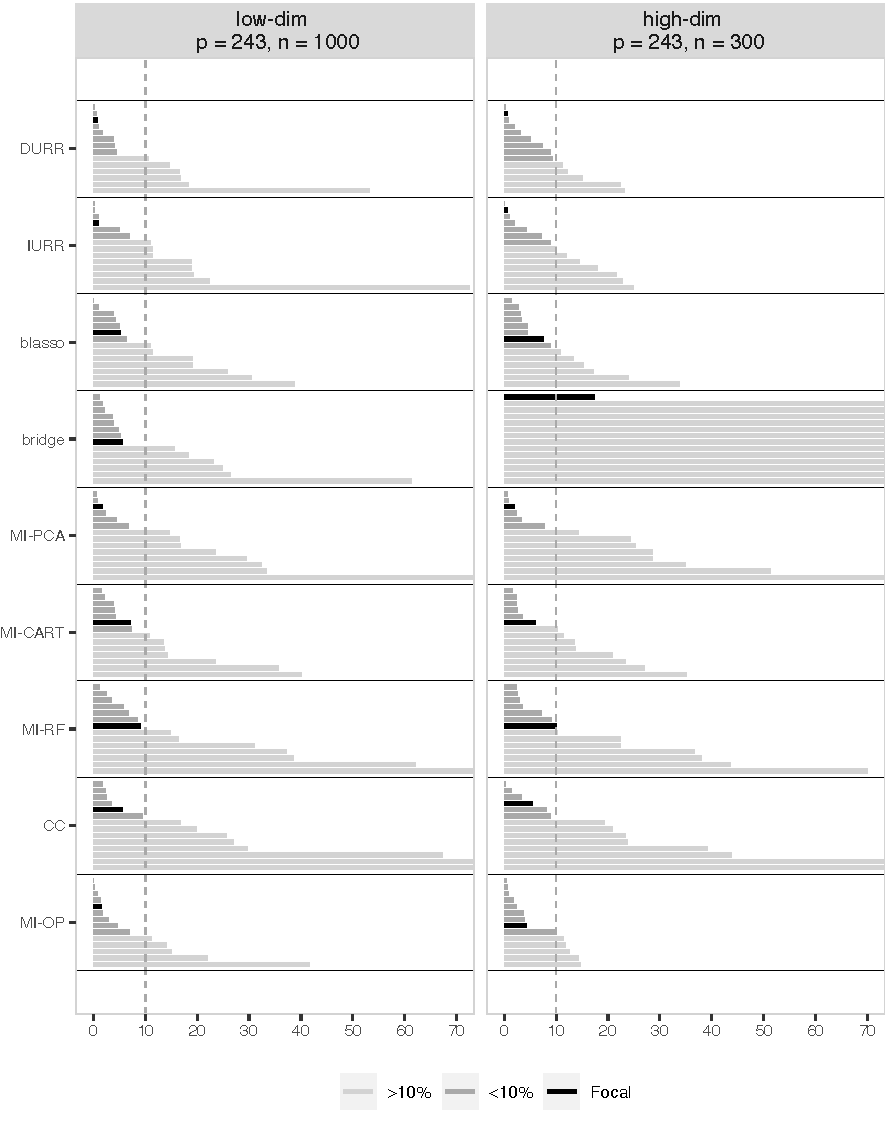
\includegraphics{\pathFIG/exp4_imp_bias_allParms_m2.pdf}
	\caption{
		$|\text{PRB}|$ for all the model parameters in model 2.
		For each method, the PRBs are reported by increasing absolute value.
		The $|\text{PRB}|$ for the focal parameter estimate is reported in black.
	}
		\label{fig:exp4_bias_allP}
\end{figure}

\begin{figure}
	\centering
	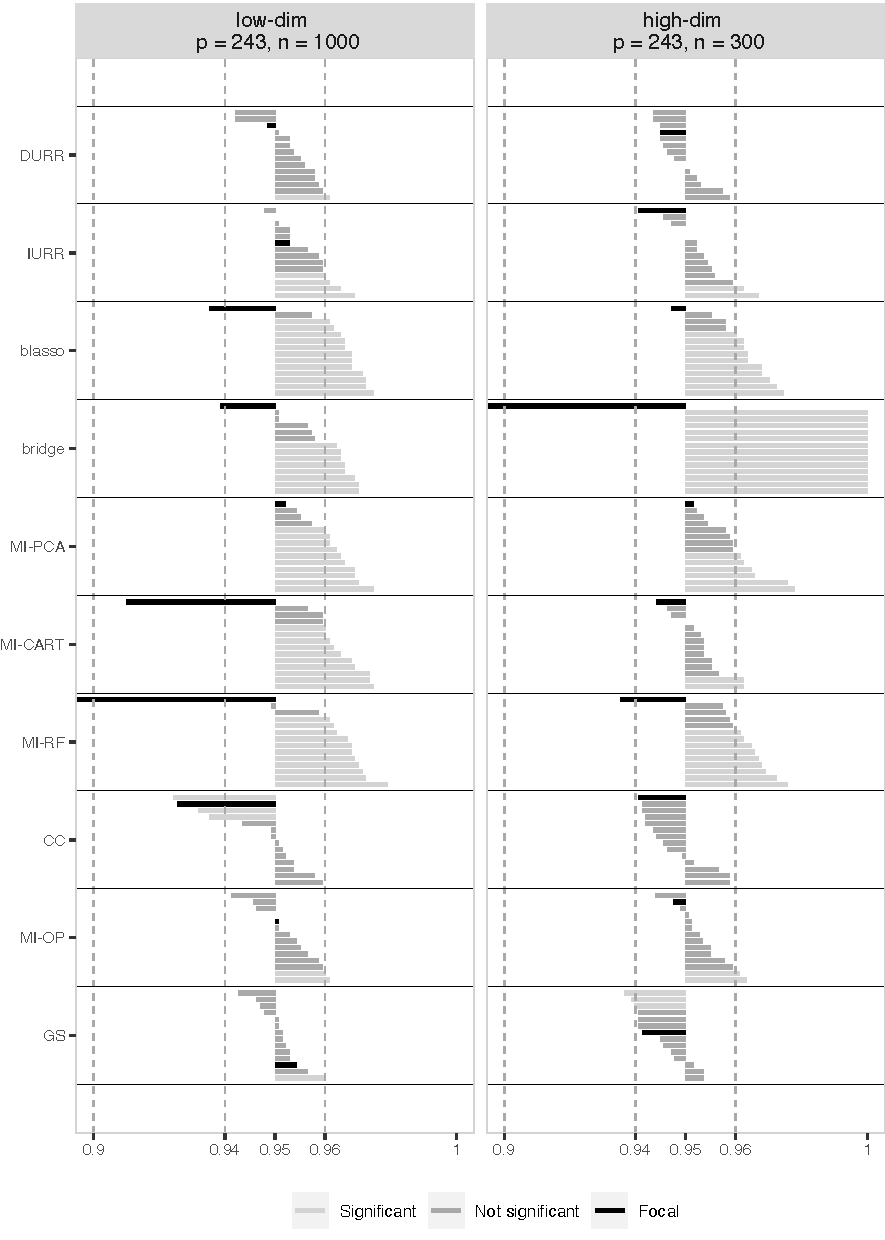
\includegraphics{\pathFIG/exp4_imp_ci_allParms_m2.pdf}
	\caption{
		CIC for all model parameters in model 2.
		For each method, the CICs are reported by increasing value.
		The CIC of the focal parameter is reported in black.
	}
	\label{fig:exp4_ci_allP}
\end{figure}

\FloatBarrier

\subsubsection{Imputation time}

	Table \ref{tab:time} reports the average imputation time for the different methods.
	IURR and DURR were the most time-consuming methods, with imputation times above one hour 
	in the low-dimensional condition. 
	MI-PCA and blasso had imputation times of a minute or less.
	In the high-dimensional condition, IURR and DURR were not as time-intensive due to the smaller
	sample size but still took more than ten times longer than MI-PCA and blasso.

\begin{table}
\tbl{Average imputation time in minutes for the MI methods compared in Experiment 3.}
	{
	\begin{tabular}{l c c c c c c c c} 
		\toprule
		condition & DURR & IURR & blasso & bridge & MI-PCA & MI-CART & MI-RF & MI-OP \\
		\midrule
		low-dim (n = 1000) & 73.20 & 75.90 & 1.40 & 8.10 & 0.60 & 4.00 & 11.30 & 2.20 \\ 
		high-dim (n = 300) & 6.10 & 9.70 & 0.50 & 3.20 & 0.40 & 1.40 & 4.70 & 1.90 \\	
		\bottomrule
	\end{tabular}
	}
\tabnote{\textsuperscript{a} In both conditions, the number of data columns was 243; $n$ refers to the 
	sample size.}
\label{tab:time}
\end{table}

\FloatBarrier


